\documentclass[10pt]{beamer}

%packages
\usepackage{babel}
\usepackage[utf8]{inputenc}
\usepackage{amsmath,tabu}
\usepackage{color}
\usepackage{tikz}
\usetikzlibrary{matrix,chains,positioning,decorations.pathreplacing,arrows}
\usetikzlibrary{calc,shadings}
\usepackage{pgfplots}
\usepackage{colortbl}
\usepackage{eurosym}
\usepackage{mathtools}
\usepackage{listings}

%definitions
\usepackage{algorithm,algorithmic}

%theme
\usetheme{Dresden}
\usecolortheme{rose}
\useoutertheme{tree}

%environments
\newenvironment{ExampleGer}{\begin{exampleblock}{Beispiel}}{\end{exampleblock}}

\newenvironment{customlegend}[1][]{%
	\begingroup
	% inits/clears the lists (which might be populated from previous
	% axes):
	\csname pgfplots@init@cleared@structures\endcsname
	\pgfplotsset{#1}%
}{%
	% draws the legend:
	\csname pgfplots@createlegend\endcsname
	\endgroup
}%

%definitions
\def\addlegendimage{\csname pgfplots@addlegendimage\endcsname}
% definition to insert numbers
\pgfkeys{/pgfplots/number in legend/.style={%
		/pgfplots/legend image code/.code={%
			\node at (0.295,-0.0225){#1};
		},%
	},
}

%general
\title{A Deep Neural Network Approach to Splice Site Prediction}
\author{Tilman Hinnerichs}
\institute{Knowledge Mining Lab -- KAUST}
\date{October 13, 2019}

%presentation
\expandafter\def\expandafter\insertshorttitle\expandafter{%
	\insertshorttitle\hspace{7cm}%
	\insertframenumber\,/\,\inserttotalframenumber
}
\begin{document}
	
\begin{frame}
	\titlepage
\end{frame}

\begin{frame}{Outline}
	\setbeamertemplate{section in toc}[sections numbered]
	\tableofcontents
\end{frame}

\section{Problem Description}
\begin{frame}{Problem Description}
	\begin{figure}[ht]
		\centering
		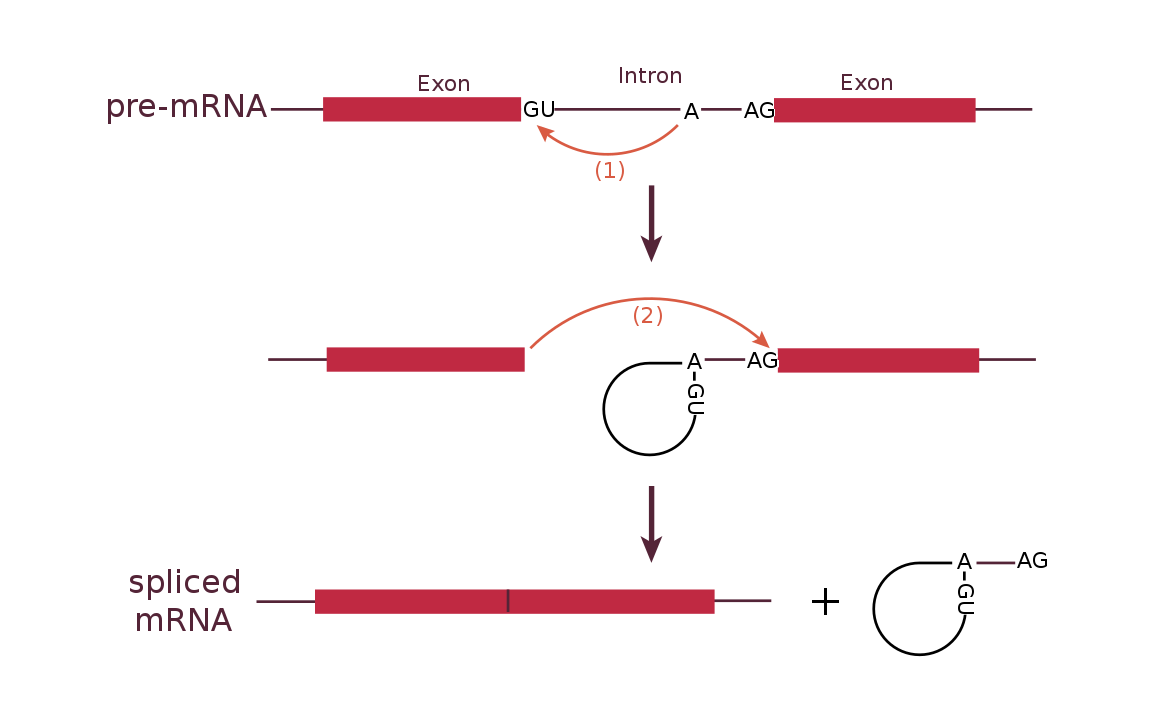
\includegraphics[width = 0.85\textwidth]{RNA_splicing_reaction.png}
		\caption{RNA splicing reaction (en.wikipedia.org)}
	\end{figure}
\end{frame}

\begin{frame}{Problem Description}
	
	\large Splice site prediction on Arabidopsis thaliana genome
	\vspace{0.5cm}
	\pause
	\begin{exampleblock}{}
		\begin{itemize}
			\item Acceptor site:\\
			\dots CGTATCT\only{\colorbox{green}}<3->{AG}ATG\only{\colorbox{red}}<4->{AG}CA\dots
			\item Donor site:\\
			\dots ATGATTT\only{\colorbox{green}}<3->{GT}GCA\only{\colorbox{red}}<4->{GT}CA\dots
			
		\end{itemize}
	\end{exampleblock}
	
\end{frame}

\section{Dataset description}
\begin{frame}{Dataset description}
	
	\large Example file, e.g., acceptor site
	\begin{align*}
	\begin{bmatrix}
	CT \dots \rotatebox{0}{\footnotesize $ 300 $ nt} \dots AG \dots \rotatebox{0}{\footnotesize $ 300 $ nt} \dots GC\\
	AG \dots \rotatebox{0}{\footnotesize $ 300 $ nt} \dots AG \dots \rotatebox{0}{\footnotesize $ 300 $ nt} \dots TT \\
	GA \dots \rotatebox{0}{\footnotesize $ 300 $ nt} \dots AG \dots \rotatebox{0}{\footnotesize $ 300 $ nt} \dots AA \\[0.2ex]
	\vdots\\
	\rotatebox{90}{\footnotesize$ ~100,000 $ records} \\[-1.3ex]
	\vdots \\[1.4ex]
	TT \dots \rotatebox{0}{\footnotesize $ 300 $ nt} \dots AG \dots \rotatebox{0}{\footnotesize $ 300 $ nt} \dots CC
	\end{bmatrix}
	\end{align*}
\end{frame}

\section{Simple classifiers}
\begin{frame}{Simple non-convolutional NN}
	\begin{itemize}
		\item Models built on one-hot-encoded data
		\item Dense networks with dropout
	\end{itemize}
	\begin{figure}
		\centering
		\begingroup
		\def\arraystretch{1.2}
		\begin{tabular}{|l|r|r|r|r|}
			\hline
			Approach & Samples & Depth & Acceptor acc. & Donor acc. \\
			\hline
			DNN & 20,000 & 7 & 92.38 & 93.43 \\
			DNN & 200,000 & 7 & 93.34 & 93.34 \\
			\hline  
		\end{tabular}
		\endgroup
		\caption{Binary classification results}
	\end{figure}
\end{frame}

\section{DiProDB database}

\subsection{Application of CNN}
\begin{frame}{Application of CNN to the DiProDB data}
	\begin{itemize}
		\item DiProDB is database for the physicochemical properties of dinucleotides (127 entries)
		\item Applied PCA yielding 15 dimensions
	\end{itemize}
	\pause
	\begin{figure}
		\small
		\centering
		\begingroup
		\def\arraystretch{1.2}
		\begin{tabular}{|l|r|r|r|r|r|r|r|r|}
			\hline
			Approach  & \multicolumn{2}{c}{Layers} & \multicolumn{3}{|c|}{Acceptor} & \multicolumn{3}{c|}{Donor} \\
			\cline{2-9}
			&Conv. & Others & Acc. & Prec. & Rec. & Acc. & Prec. & Rec. \\
			\hline
			CNN DPDB & 4 & 5 & 94.4 & 95.4 & 94.6 & 94.9 & 94.4 & 94.7 \\
			CNN DPDB & 4 & 7 & 93.5 & 93.3 & 94.5 & 94.0 & 94.0 & 93.3 \\
			CNN DPDB & 6 & 5 & 94.0 & 93.9 & 94.9 & 94.2 & 95.4 & 91.6 \\
			CNN DPDB & 6 & 5 & 94.4 & 97.0 & 93.8 & 95.2 & 96.5 & 93.7 \\
			SpliceRover & 4 & 2 & 96.1 & 93.9 & 97.4 & 95.4 & 95.6 & 96.7 \\
			CNN DPDB(*) & 2 & 4 & 94.3 & 95.6 & 94.3 & 95.3 & 96.9 & 94.4 \\
			
			\hline  
		\end{tabular}
		\endgroup
	\end{figure}
	SpliceRover[Zuallaert et al., 2018]
\end{frame}

\begin{frame}
	\begin{figure}[ht]
		\centering
		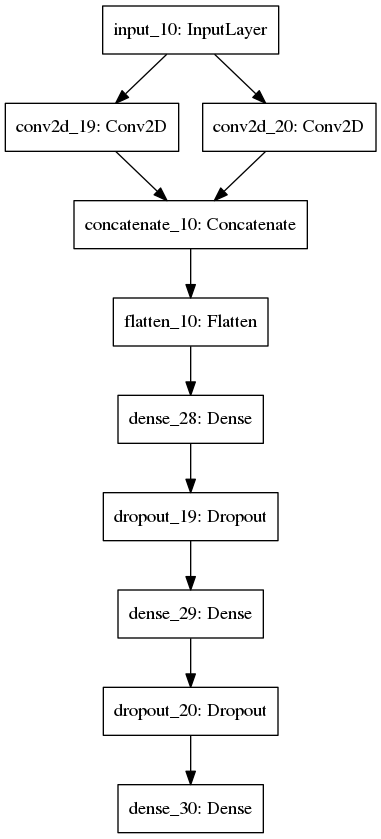
\includegraphics[width = 0.65\textwidth]{../../models/plotted_models/DiProDB_model.png}
	\end{figure}
\end{frame}

\section{Improvements on simple approach}
\begin{frame}{Improvements on simple approach}
	Applying convolutional models to one hot encoding of
	\begin{itemize}
		\item single nucleotides
		\begin{figure}
			\small
			\centering
			\begingroup
			\def\arraystretch{1.2}
			\begin{tabular}{|l|r|r|r|r|r|r|r|}
				\hline
				Approach  & Samples & \multicolumn{3}{c|}{Acceptor} & \multicolumn{3}{c|}{Donor} \\
				\cline{3-8}
				& & Acc. & Prec. & Rec. & Acc. & Prec. & Rec. \\
				\hline
				Simple & 200000 & 94.5 & 95.6 & 93.3 & 95.3 & 96.7 & 94.5 \\
				
				\hline  
			\end{tabular}
			\endgroup
		\end{figure}
		\item trinucleotides
		\begin{figure}
			\small
			\centering
			\begingroup
			\def\arraystretch{1.2}
			\begin{tabular}{|l|r|r|r|r|r|r|r|}
				\hline
				Approach  & Samples & \multicolumn{3}{c|}{Acceptor} & \multicolumn{3}{c|}{Donor} \\
				\cline{3-8}
				& & Acc. & Prec. & Rec. & Acc. & Prec. & Rec. \\
				\hline
				Simple & 40000 & 94.6 & 93.3 & 96.7 & 95.0 & 92.5 & 96.3 \\
				Simple & 200000 & 95.6 & 96.6 & 94.6 & 95.8 & 96.7 & 95.0\\
				
				\hline  
			\end{tabular}
			\endgroup
		\end{figure}
	\end{itemize}
\end{frame}

\begin{frame}{Single nucleotides model}
	\begin{figure}[ht]
		\centering
		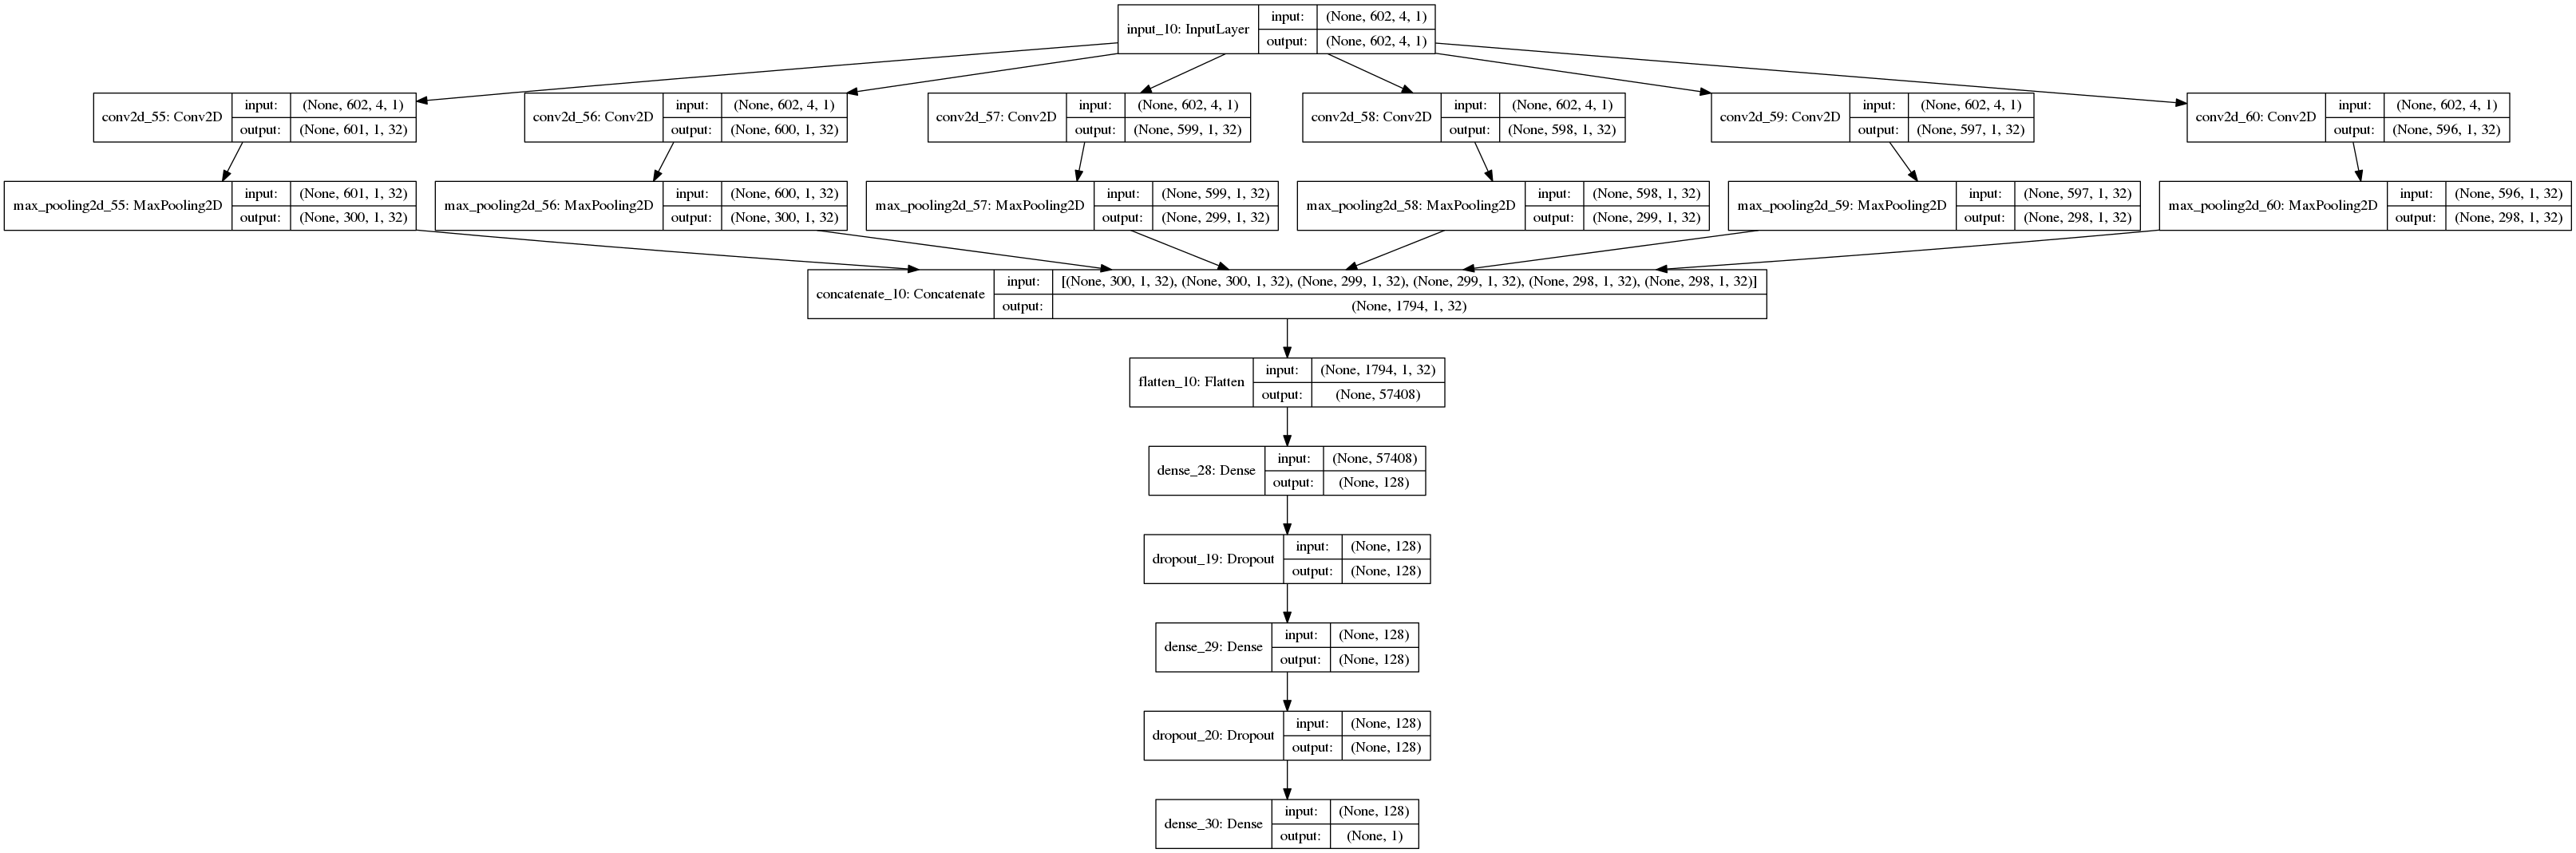
\includegraphics[width = 1.05\textwidth]{../../models/plotted_models/simple_model.png}
		\caption{Convolutional model with filter sizes (2x4), \dots, (7x4)}
	\end{figure}
\end{frame}

\begin{frame}{Trinucleotides model}
	\begin{figure}[ht]
		\centering
		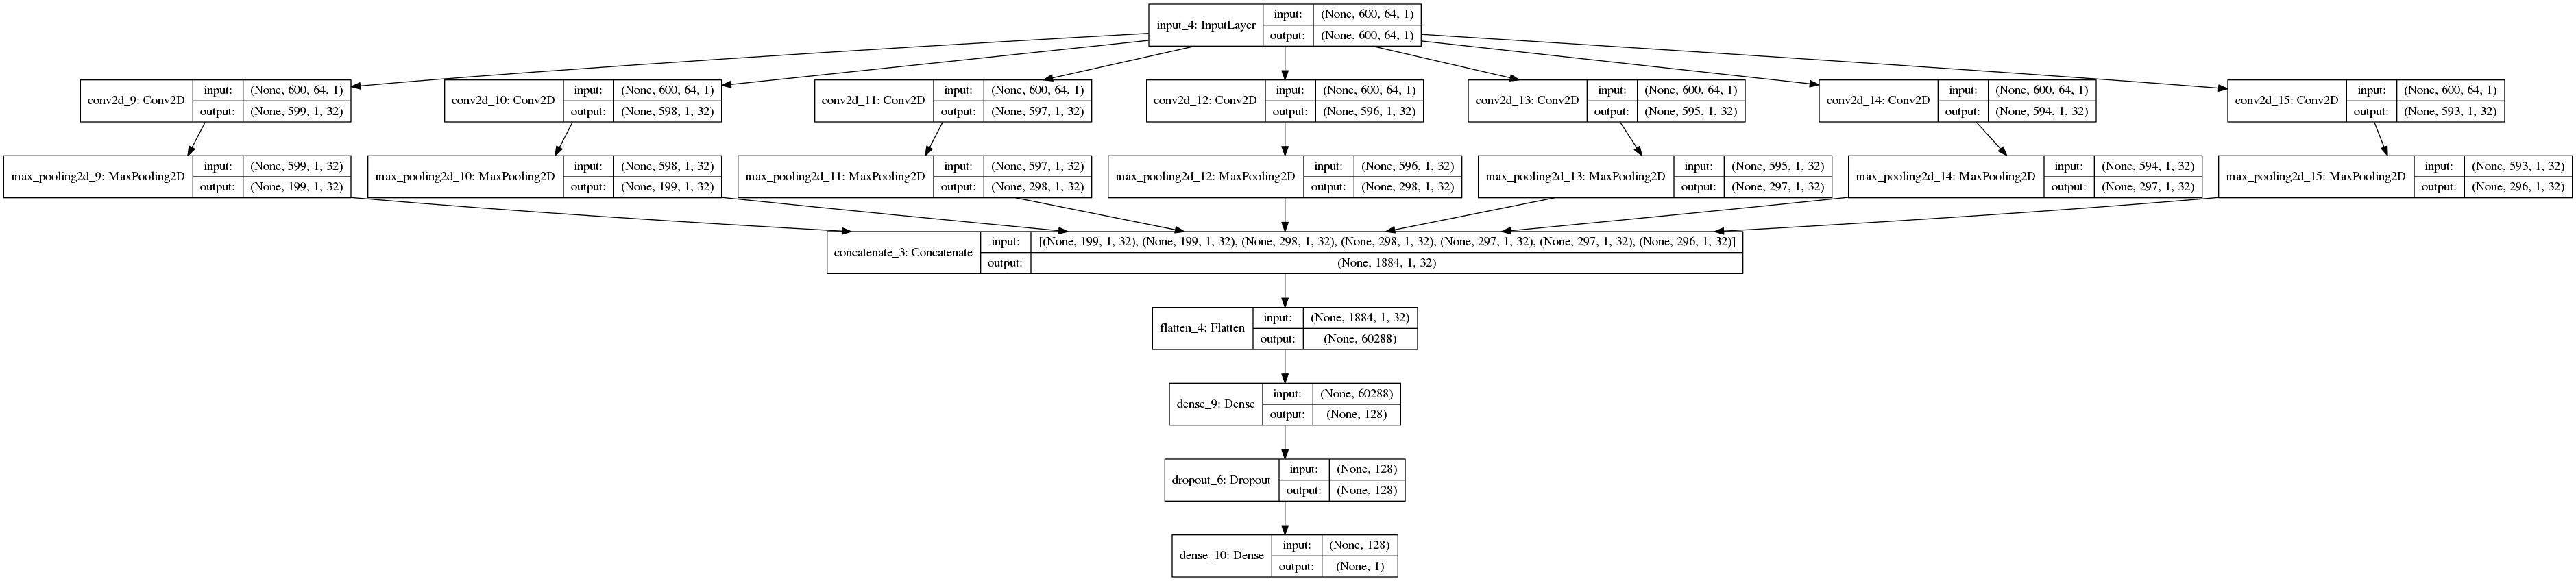
\includegraphics[width = 1.05\textwidth]{../../models/plotted_models/trint_model_2019-10-08_09-27-12.png}
		\caption{Convolutional model with filter sizes (2 x 64), \dots, (8x64)}
	\end{figure}
\end{frame}

\section{repDNA}
\begin{frame}{repDNA (Liu, 2014)}
	A \glqq Python package to generate various modes of feature vectors for DNA sequences\grqq:
	\begin{block}{repDNA content}
		\begin{itemize}
			\item Nucleic acid composition
			\begin{itemize}
				\item kmer
				\item Increment of diversity (ID)
			\end{itemize}
			\item Autocorrelation
			\begin{itemize}
				\item Dinucleotide-based auto covariance (DAC)
				\item Dinucleotide-based cross covariance (DCC)
				\item Dinucleotide-based auto-cross covariance (DACC)
				\item Trinucleotide-based auto covariance (TAC)
				\item Trinucleotide-based cross covariance (TCC)
				\item Trinucleotide-based auto-cross covariance (TACC)
			\end{itemize}
		\end{itemize}
	\end{block}
\end{frame}

\begin{frame}{repDNA (Liu, 2014)}
	\begin{block}{repDNA content}
		\begin{itemize}
			\item Pseudo nucleotide composition
			\begin{itemize}
				\item Pseudo dinucleotide composition (PseDNC)
				\item Pseudo k-tupler nucleotide composition (PseKNC)
				\item Parallel correlation pseudo dinucleotide composition (PC-PseDNC)
				\item Parallel correlation pseudo trinucleotide composition (PC-PseTNC)
				\item Series correlation pseudo dinucleotide composition (SC-PseDNC)
				\item Series correlation pseudo trinucleotide composition (SC-PseTNC)
			\end{itemize}
		\end{itemize}
	\end{block}
	\pause
	\begin{itemize}
		\item Build model for each encoding and reuse filters for overall model
	\end{itemize}
\end{frame}

\begin{frame}{Classifier model on repDNA features: Results}
	\begin{figure}
		\small
		\centering
		\begingroup
		\def\arraystretch{1.2}
		\begin{tabular}{|l|r|r|r|r|r|r|r|}
			\hline
			Approach  & Samples & \multicolumn{3}{c|}{Acceptor} & \multicolumn{3}{c|}{Donor} \\
			\cline{3-8}
			& & Acc. & Prec. & Rec. & Acc. & Prec. & Rec. \\
			\hline
			IDkmer & 200000 & 75.2 & 72.3 & 76.7 & 72.7 & 77.05 & 75.6 \\
			DAC & 200000 & 75.5 & 72.8 & 77.0 & 75.2 & 68.9 & 78.8 \\
			DCC & 200000 & 75.1 & 80.0 & 77.7 & 74.5 & 75.2 & 80.0 \\
			TAC & 200000 & 68.0 & 58.3 & 72.4 & 68.2 & 57.1 & 73.3 \\
			TCC & 200000 & 73.6 & 75.5 & 72.7 & 75.3 & 65.0 & 82.0 \\
			PseKNC & 200000 & 78.1 & 76.0 & 79.4 & 75.84 & 71.3 & 78.4 \\
			PC-PseDNC & 200000 & 78.0 & 76.5 & 80.1 & 76.4 & 75.1 & 77.9 \\
			PC-PseTNC & 200000 & 80.5 & 76.1 & 84.2 & 78.8 & 76.9 & 81.6 \\
			SC-PseDNC & 200000 & 79.2 & 74.5 & 82.4 & 77.5 & 77.0 & 78.8 \\
			SC-PseTNC & 200000 & 80.6 & 76.3 & 84.8 & 78.7 & 77.3 & 81.5\\
			\hline  
		\end{tabular}
		\endgroup
	\end{figure}
\end{frame}

\begin{frame}{Classifier model on repDNA features: IDkmer}
	\begin{figure}[ht]
		\centering
		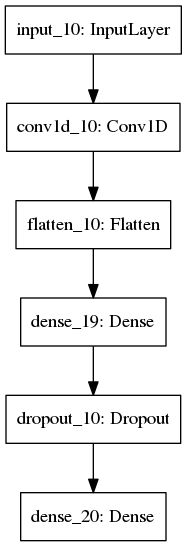
\includegraphics[width = 0.35\textwidth]{../../models/plotted_models/IDkmer_model.png}
	\end{figure}
\end{frame}

\begin{frame}{Classifier model on repDNA features: DAC/DCC/TAC/TCC}
	\begin{figure}[ht]
		\centering
		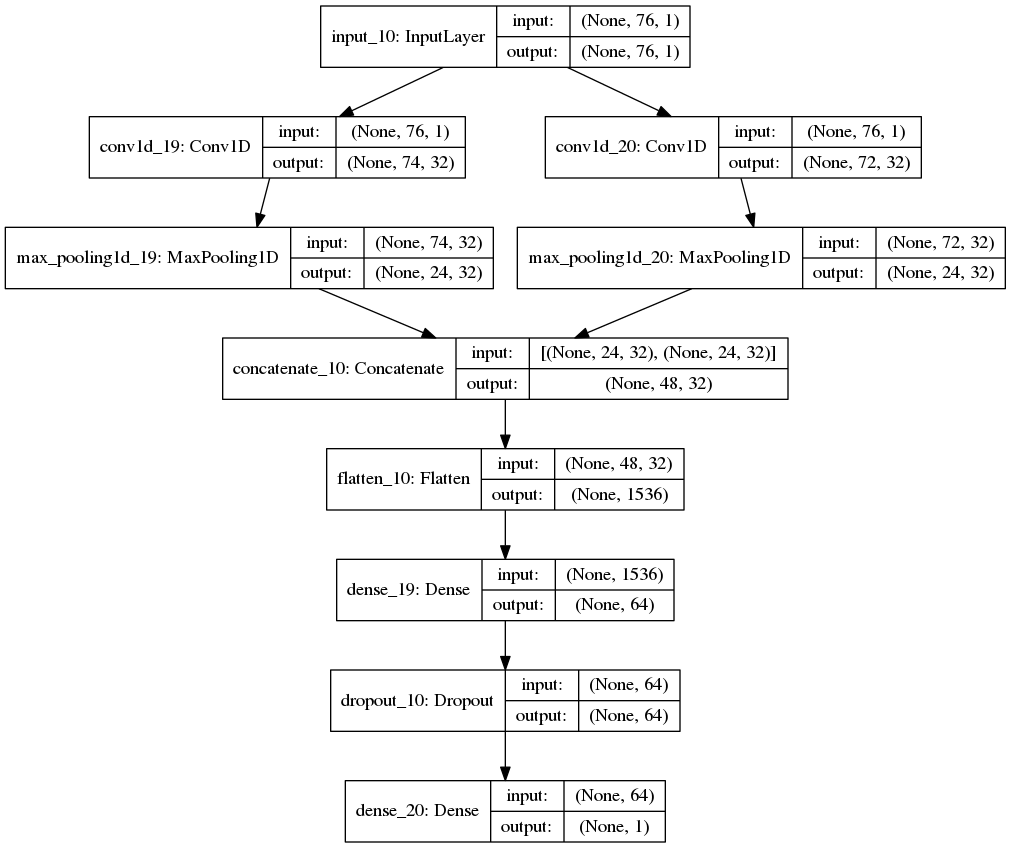
\includegraphics[width = 0.75\textwidth]{../../models/plotted_models/dac_model.png}
	\end{figure}
\end{frame}

\begin{frame}{Classifier model on repDNA features: PseNAC}
	\begin{figure}[ht]
		\centering
		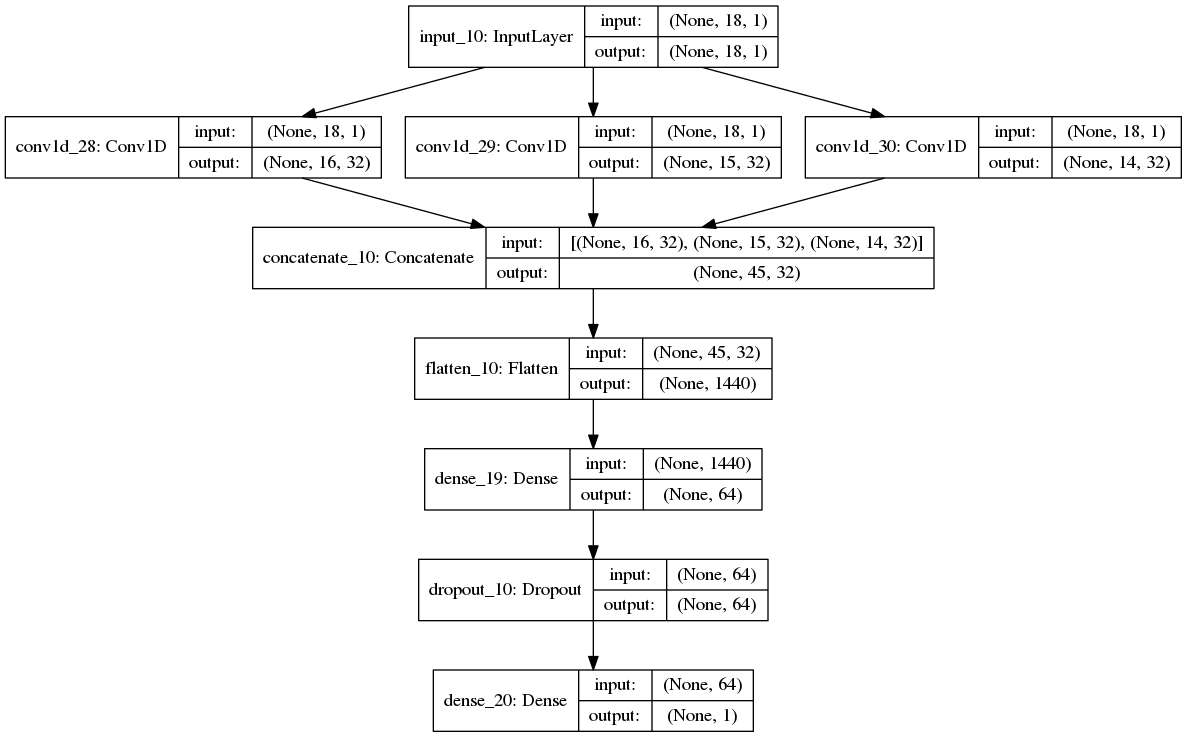
\includegraphics[width = 0.95\textwidth]{../../models/plotted_models/PC_PseDNC_model.png}
	\end{figure}
\end{frame}

\begin{frame}{Additional models}
	\begin{itemize}
		\item XGBoost: Library for gradient boosting algorithms
		\item Random Forest
	\end{itemize}
	\pause
	\begin{figure}
		\small
		\centering
		\begingroup
		\def\arraystretch{1.2}
		\begin{tabular}{|l|r|r|r|r|r|r|}
			\hline
			Approach  & \multicolumn{3}{c|}{Acceptor} & \multicolumn{3}{c|}{Donor} \\
			\cline{2-7}
			 & Acc. & Prec. & Rec. & Acc. & Prec. & Rec. \\
			\hline
			XGBoost  & 90.8 & 89.5 & 92.0 & 92.0 & 90.6 & 93.3 \\
			Random Forest & 83.5 & 83.0 & 83.8 & 86.0 & 86.3 & 85.8\\
			\hline  
		\end{tabular}
		\endgroup
	\end{figure}
\end{frame}

\subsection{Funnel}
\begin{frame}{Funneling method: Model}
	\begin{figure}[ht]
		\centering
		\tikzset{%
			every neuron/.style={
				circle,
				draw,
				minimum size=0.3cm
			},
			neuron missing/.style={
				draw=none, 
				scale=4,
				text height=0.333cm,
				execute at begin node=\color{black}$\vdots$
			},
		}
		
		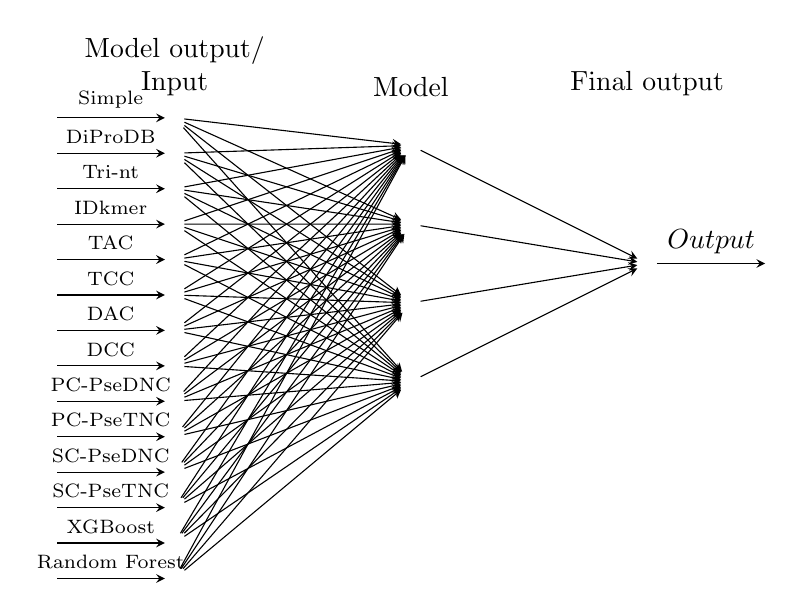
\begin{tikzpicture}[x=1.5cm, y=1.0cm, >=stealth]
		
		\foreach \m/\l [count=\y] in {1,2,3,4,5,6,7,8,9,10,11,12,13,14}
		\node [every neuron/.try, neuron \m/.try] (input-\m) at (0,2.3-0.45*\y) {};
		
		\foreach \m [count=\y] in {1,2,3,4}
		\node [every neuron/.try, neuron \m/.try ] (hidden-\m) at (2,2.5-\y) {};
		
		\foreach \m [count=\y] in {1}
		\node [every neuron/.try, neuron \m/.try ] (output-\m) at (4,0) {};
		
		%\foreach \l [count=\i] in {1, 2,3,4,5,6,7,8,9,10}
		%\draw [<-] (input-\i) -- ++(-1,0)
		%node [above, midway] {$I_{\l}$};
		
		\draw [<-] (input-1) -- ++(-1,0)
		node [above, midway] {\scriptsize Simple};
		\draw [<-] (input-2) -- ++(-1,0)
		node [above, midway] {\scriptsize DiProDB};
		\draw [<-] (input-3) -- ++(-1,0)
		node [above, midway] {\scriptsize Tri-nt};
		\draw [<-] (input-4) -- ++(-1,0)
		node [above, midway] {\scriptsize IDkmer};
		\draw [<-] (input-5) -- ++(-1,0)
		node [above, midway] {\scriptsize TAC};
		\draw [<-] (input-6) -- ++(-1,0)
		node [above, midway] {\scriptsize TCC};
		\draw [<-] (input-7) -- ++(-1,0)
		node [above, midway] {\scriptsize DAC};
		\draw [<-] (input-8) -- ++(-1,0)
		node [above, midway] {\scriptsize DCC};
		\draw [<-] (input-9) -- ++(-1,0)
		node [above, midway] {\scriptsize PC-PseDNC};
		\draw [<-] (input-10) -- ++(-1,0)
		node [above, midway] {\scriptsize PC-PseTNC};
		\draw [<-] (input-11) -- ++(-1,0)
		node [above, midway] {\scriptsize SC-PseDNC};
		\draw [<-] (input-12) -- ++(-1,0)
		node [above, midway] {\scriptsize SC-PseTNC};
		\draw [<-] (input-13) -- ++(-1,0)
		node [above, midway] {\scriptsize XGBoost};
		\draw [<-] (input-14) -- ++(-1,0)
		node [above, midway] {\scriptsize Random Forest};
		
		
		\foreach \l [count=\i] in {1}
		\draw [->] (output-\i) -- ++(1,0)
		node [above, midway] {$Output$};
		
		\foreach \i in {1,...,14}
		\foreach \j in {1,...,4}
		\draw [->] (input-\i) -- (hidden-\j);
		
		\foreach \i in {1,...,4}
		\foreach \j in {1,...,1}
		\draw [->] (hidden-\i) -- (output-\j);
		
		%\foreach \l [count=\x from 0] in {Input, Hidden, Ouput}
		\node [align=center, above] at (0*2,2) {Model output/\\Input};
		\node [align=center, above] at (1*2,2) {Model};
		\node [align=center, above] at (2*2,2) {Final output};

		\end{tikzpicture}
	\end{figure}
\end{frame}

\begin{frame}{Funneling method: Soft vote results}
	\begin{itemize}
		\item Random search on weighted filters
	\end{itemize}
	\begin{figure}
		\scriptsize
		\centering
		\begingroup
		\def\arraystretch{1.1}
		\begin{tabular}{|l|r|r|r|r|r|r|r|r|r|r|r|r|r|}
			\hline
			& \multicolumn{7}{|c|}{Weights} & \multicolumn{6}{c|}{Results}\\
			\hline
			M & S & D & T & R & X & dc & Ps& \multicolumn{3}{c|}{Acceptor} & \multicolumn{3}{c|}{Donor} \\
			\cline{9-14}
			&&&&&&& & Acc. & Prec. & Rec. & Acc. & Prec. & Rec. \\
			\hline
			S &1&0&1&0&0&0&0 & 95.5 & 96.0 & 95.0 & 96.0 & 96.9 & 95.2 \\
			H &1&0&1&0&0&0&0 & 95.1 & 97.5 & 93.1 & 95.5 & 97.9 & 93.5 \\
			S &1&1&3&1&1&0&0 & 95.2 & 95.5 & 95.0 & 95.8 & 96.2 & 95.3 \\
			H &1&1&3&1&1&0&0 & 95.5 & 96.6 & 94.6 & 95.9 & 97.1 & 94.9 \\
			
			S &3&2&3&2&1&0&0 & 95.0 & 95.1 & 94.9 & 95.7 & 96.2 & 95.2 \\
			H &3&2&3&2&1&0&0 & 95.2 & 95.6 & 94.9 & 95.8 & 96.5 & 95.1 \\
			S &8&5&8&2&0&0&0 & 95.4 & 95.8 & 95.1 & 95.9 & 96.6 & 95.3 \\
			H &8&5&8&2&0&0&0 & 95.4 & 96.3 & 94.7 & 95.9 & 97.0 & 94.9 \\
			 
			\hline 
		\end{tabular}
		\endgroup
	\end{figure}
\end{frame}

\begin{frame}{Funneling method: Soft vote results}
	\begin{itemize}
		\item Random search on weighted filters
	\end{itemize}
	\begin{figure}
		\scriptsize
		\centering
		\begingroup
		\def\arraystretch{1.1}
		\begin{tabular}{|l|r|r|r|r|r|r|r|r|r|r|r|r|r|}
			\hline
			& \multicolumn{7}{|c|}{Weights} & \multicolumn{6}{c|}{Results}\\
			\hline
			 M & S & D & T & R & X & dc & Ps& \multicolumn{3}{c|}{Acceptor} & \multicolumn{3}{c|}{Donor} \\
			\cline{9-14}
			&&&&&&& & Acc. & Prec. & Rec. & Acc. & Prec. & Rec. \\
			\hline
			S & 1 & 1 & 1 & 1 & 1 & 1 & 1 & 92.0 & 90.3 & 92.4 &94.1 & 93.9 & 94.4\\
			H& 1 & 1 & 1 & 1 & 1 & 1 & 1 & 85.0 & 80.3 & 88.5 & 85.8 & 80.7 & 89.8\\	
			S & 5&2&5&4&4&1&1& 94.8 & 94.9 & 94.8 & 95.6 & 95.9 & 95.2\\
			H&5&2&5&4&4&1&1&95.1 & 95.7 &94.6 & 95.8 & 96.5 & 95.1\\	
			S & 5&5&5&4&4&1&1 & 95.1 & 95.2 & 95.0 & 95.8 & 96.3 & 95.4 \\
			H & 5&5&5&4&4&1&1 & 95.3 & 95.5 & 95.0 & 95.9 & 96.5 & 95.3 \\
			S & 7&7&7&5&5&1&1 & 95.2 & 95.3 & 95.1 & 95.8 & 96.3 & 95.3 \\
			H & 7&7&7&5&5&1&1 & 95.3 & 95.7 & 95.0 & 96.0 & 96.6 & 95.3 \\
			S & 7&7&7&5&0&0&0 & 95.3 & 95.6 & 95.0 & 95.8 & 96.5 & 95.2 \\
			H & 7&7&7&5&0&0&0 & 95.5 & 96.1 & 95.0 & 96.0 & 96.9 & 95.1 \\
			S & 95&95&95&90&85&80&80 & 93.7 & 92.9 & 94.3 & 94.9 & 95.0 & 94.8 \\
			H & 95&95&95&90&85&80&80 & 86.7 & 82.9 & 89.1 & 84.8 & 80.72 & 90.0 \\
				
			\hline 
		\end{tabular}
		\endgroup
	\end{figure}
\end{frame}

\begin{frame}{Funneling method: Results}
	Minimization techniques:
	\begin{itemize}
		\item Nalder-Mead
		\item Powell
	\end{itemize}
	\pause
	\begin{figure}
		\small
		\centering
		\begingroup
		\def\arraystretch{1.2}
		\begin{tabular}{|l|r|r|r|r|r|r|}
			\hline
			Approach  & \multicolumn{3}{c|}{Acceptor} & \multicolumn{3}{c|}{Donor} \\
			\cline{2-7}
			& Acc. & Prec. & Rec. & Acc. & Prec. & Rec. \\
			\hline
			Soft Min. & 83.8 & 83.5 & 83.0 & 86.0 & 86.3 & 85.8 \\
			Hard Min. & 83.5 & 83.0 & 84.1 & 86.5 & 86.7 & 86.3 \\
			\hline 
			\pause
			Grad boost & 83.5 & 83.0 & 83.8 & 86.0 & 86.3 & 85.8 \\
			Random Forest & 93.7 & 94.2 & 93.3 & 94.1 & 94.9 & 93.4 \\
			NN & 83.5 & 83.0 &83.8 & 87.0 & 85.5 & 87.4 \\
			Naive Bayes & 83.5 & 83.0 & 83.8 & 85.9 & 86.3 & 85.8 \\
			\hline
		\end{tabular}
		\endgroup
	\end{figure}
\end{frame}

\begin{frame}{Citations}
	\footnotesize
	\begin{itemize}
		\item Liu B, Liu F, Fang L, Wang X, Chou K-C.repDNA: a Python package to generate various modes of feature vectors for DNA sequences by incorporating user-defined physicochemical properties and sequence-order effects. Bioinformatics 2015;31(8):1307-1309.
		\item Jasper Zuallaert, Fréderic Godin, Mijung Kim, Arne Soete, Yvan Saeys, Wesley De Neve, SpliceRover: interpretable convolutional neural networks for improved splice site prediction, Bioinformatics, Volume 34, Issue 24, 15 December 2018, Pages 4180–4188, https://doi.org/10.1093/bioinformatics/bty497
	\end{itemize}
\end{frame}

\end{document}